\section{Implementation and Evaluation}
\label{sec:evaluation}

The Alloy case study uses the Alloy~6 parser, Kodkod, SAT4J and Pardinus.
The supervised run completed on 27 November 2026 UTC from commit \texttt{9693595e}.
It covers the paired corpus, full reference pools, natural ablation,
controlled capability suite and natural slot-typing comparison. The
synthetic scaling grid comes from the earlier v3 experiment.

\subsection{Implementation and experimental setup}
\label{sec:eval-setup}

\paragraph{Two \CanDis{} implementations and shared ablation baselines.}
Our codebase maintains two implementations of \CanDis{} that share the repaired
source normalization rules and established repair distance metric:
\begin{itemize}
\item \textbf{Fast Rewrite IR} executes the staged temporal, prenex, and
  slotted normalization pipeline directly alongside the reference repair metric
  for high-throughput analysis.
\item \textbf{Certificate-Integrated IR} reconstructs the typed flexible-arity
  slotted e-graph with in-process certificate construction, strict
  per-transition invariant checks, congruence rebuilding, and bounded
  finite-unfolding observation.
\end{itemize}
Both implementations selected the same structural zeros on the paired
corpus and correct-reference pools and gave equal scalar scores for all
1,894,168 positive-distance ranking comparisons. We report their shared
effectiveness and measure each implementation's resource use separately.

To isolate representation choices, we compare \CanDis{} against five distinct
ablation baselines sharing a common bounded explicit-law rewrite frontier
(\texttt{canonical-equivalences-v3-explicit-laws}): \textbf{Raw} (fixed-arity
AST-like e-nodes), \textbf{Raw + De Bruijn} (nameless bound indices),
\textbf{Java egglog} (variadic constructors and semi-naive congruence rounds),
\textbf{Java egglog + De Bruijn}, and \textbf{Slotted} (untyped slotted
invocations and permutation groups). Variant names identify internal pipeline
configurations, not external systems.

\paragraph{Views and repair distance.}
For equality recognition, \CanDis{} compares deterministic finite-term keys.
For structural proximity when equality fails ($d>0$), the separate
\emph{repair projection} omits proof metadata and decomposes a formula $\varphi$
into its temporal skeleton $T_\varphi$, phase-local binding view $B_\varphi$,
and normalized matrix $M_\varphi$:
\[
 d_{\mathrm{repair}}(\varphi,\psi)=
 d_{\mathrm{temp}}(T_\varphi,T_\psi)+
 d_{\mathrm{quant}}(B_\varphi,B_\psi)+
 d_{\mathrm{matrix}}(M_\varphi,M_\psi),
\]
using ordered tree dynamic programming for $d_{\mathrm{temp}}$, exact
type-compatible matching over admitted binder orbits for $d_{\mathrm{quant}}$,
and carrier-appropriate matching ($\Seq$, $\Bag$, $\Set$, or singleton) for
$d_{\mathrm{matrix}}$ under a shared binder mapping across inherited phases.

\paragraph{Corpus and runtime environment.}
The Alloy4Fun snapshot~\cite{alloy4funDataset2023,alloy4fun,novice} accounts
for all 66,080 original student--oracle files across 181 invariant groups and
17 problem variants. Excluding 4,482 paired rows whose parsed ASTs are already
identical—an inherited paired-measurement convention rather than an exemption
from canonical obligations—leaves 61,598 eligible AST-distinct pairs: 19,212
labeled \texttt{CORRECT} and 42,386 labeled incorrect (21,715 both over- and
underconstrained, 8,095 overconstrained, and 12,576 underconstrained). The
natural and capability studies ran on an AMD Ryzen~9 9950X3D (32 logical
processors) with OpenJDK~17.0.21, 16 workers, an 8\,GiB JVM heap cap, and
deterministic seed \texttt{55520260811}. Throughout this section, zero distance
means both forms had distance zero under the implemented rewrite theory.

\subsection{How many distinct-AST student--oracle equivalences does \CanDis{} recognize on the natural corpus?}
\label{sec:eval-paired}

Both paths returned structural distance zero on \textbf{5,137} correct
pairs (26.74\% of 19,212) and on zero of 42,386 incorrect pairs.
The separate 4,482 AST-identical cases were excluded before measurement.

Taking the larger endpoint of each pair, mean size was 19.669 raw AST
nodes, 17.514 repair-projection units and 32.737 representative-tree
nodes. Mean paired distance was 13.471 under the repair projection,
17.087 under raw AST edits, 39.261 under Levenshtein edits, and
31.383 under representative-tree edits.

\subsection{How does canonicalization affect full-reference nearest-truth search and truth-pool consolidation?}
\label{sec:eval-augmenter}

For each of 42,386 incorrect submissions the Augmenter searched its
invariant's complete reference pool. The pools comprise 4,315 unique
student references and 181 oracles. All 1,894,168 measured ranking
comparisons had positive distance. The mean nearest distance was 12.267
under raw AST edits and 11.478 under \CanDis{}.

\begin{figure}[t]
\centering
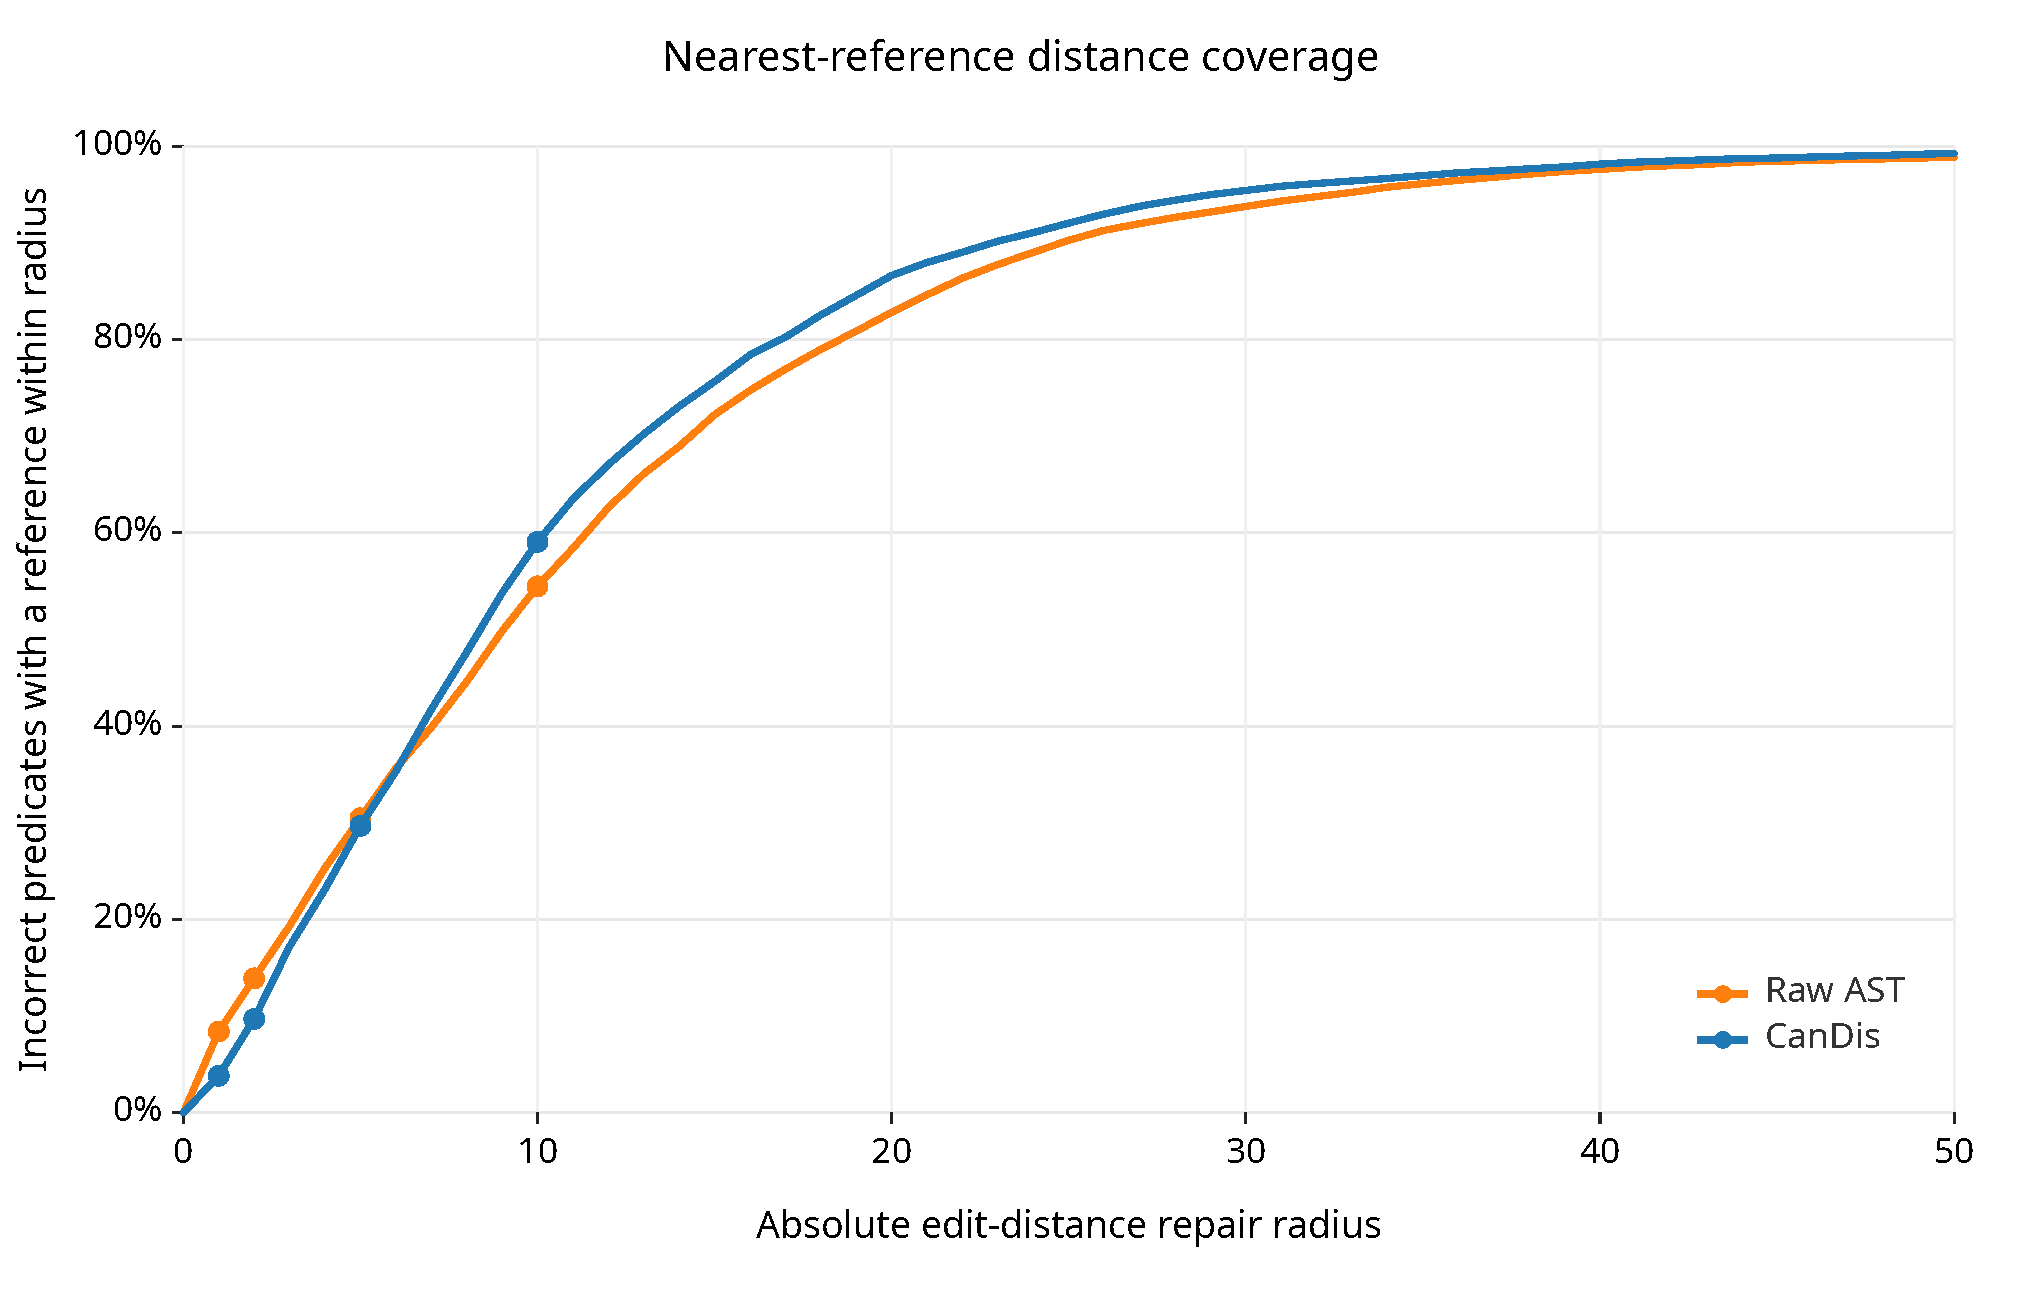
\includegraphics[width=0.82\linewidth]{figures/historical_repair_coverage.pdf}
\caption{Cumulative nearest-reference coverage for 42,386 incorrect
submissions. At an integer radius $r$, each curve counts submissions whose
nearest distinct-AST reference lies within $r$ edits under that metric.
All submissions remain in the denominator through the plotted limit of 50.}
\label{fig:distance-coverage}
\end{figure}


Figure~\ref{fig:distance-coverage} counts each submission once per metric
at each inclusive edit radius. At ten edits, 23,087 submissions had a raw-AST
reference within reach and 25,036 had a \CanDis{} reference within reach.
The two metrics can select different nearest references.

\subsection{What does checking a particular Alloy command add?}
\label{sec:scoped-pools}

A structural rewrite must hold wherever its key is reused. For instance, the
v3.1 rule moving a universal quantifier across \texttt{always} requires a
static domain: a later state must not introduce an atom that was absent at
the time of quantification. The five further rule families compare selected
relation rows or columns, bounded relation differences, ordinary and mixed
role selections, and threshold classifiers. Their conclusions need not survive
a change of command. With four-bit signed integers, for example, eight
predecessors are enough to make a count wrap negative. The test
\texttt{\#succs.t > 1} then fails although \texttt{not lone succs.t} holds.

The default comparison distinguishes structural equality from equality under
a fixed check of the two predicates. The latter test uses the resolved field,
binder and temporal frame, the effective carrier bounds and the actual integer
width. A match must produce the same witness in both orientations and the
native solver must find no counterexample. An \textsc{unsat} result without a
rule is not a new edge. For references from different files, the comparison
first checks that the relocated predicates retain their typed definitions,
imports, facts and compatible command bounds. It never substitutes a scoped
edge for an edit trace or writes that edge into the structural canonical key.

Every eligible student--oracle pair had a fixed command. A rule matched
347 pairs, recognizing 259 correct pairs beyond structural
equality. Across the 132,032 pairs of correct references every comparison
had a common command context and 1,234 pairs matched a rule.

To count \emph{structural forms}, we connect references in an invariant pool
when they have structural distance zero and count the connected components.
For \emph{fixed-command components}, we add the verified command-specific
edges and count again. A single new edge can join two entire components. The 4,496 references reduced to 1,816 structural forms
and then to 1,743 fixed-command components. Both paths recognized
all 8,952 original Slotted reference zeros and 10,319 more,
for 19,271 direct structural zeros.

\paragraph{Historical retention and native replay.}
The archives through v3.3 contain \histPublishedPaired{} distinct student--oracle
pairs and \histPublishedRefs{} direct reference pairs that reached zero in at
least one edition. Both paths retained every such pair. The regression test
checks each pair by its source and predicate identities in both engines. The 105 historical Alloy
counterexamples remained in separate fixed-command components. Seven CV
pairs had lost their shared structural form in v3.3. The repaired rules
cover these cases, including empty carriers, and each equivalence has a Lean proof.

The native checker replayed the edits selected by each engine from its
frozen normalized inputs. The ordered actions or temporal block effects
agreed on all 61,598 student--oracle comparisons, all 19,271
zero-distance reference pairs and 4,138 positive-distance ranking
comparisons selected for alternating quantifiers. Previously, completing a
partial binder map could displace an equally cheap ordinary alignment. Both
engines now break these ties by the surviving declaration positions. The
83 affected comparisons also agreed in reverse. A separate sample of one
paid comparison from each of the 181 pools agreed throughout.


\subsection{Which capabilities separate \CanDis{} from the baselines on controlled and natural predicates?}
\label{sec:eval-capability}

The seven-arm natural experiment found 5,137 correct zeros on each
\CanDis{} path, including all 2,228 Slotted zeros and 2,909
additional pairs. On the controlled suite, Slotted and both \CanDis{}
paths recognized all 5,500 transformations.

\begin{table}[t]
\centering
\caption{Natural-corpus effectiveness (19,212 correct and 42,386
incorrect distinct-AST pairs) and controlled capability coverage
(11 families of 500, including binder permutation).}

\label{tab:eval-effectiveness}
\scriptsize
\setlength{\tabcolsep}{2.7pt}
\begin{tabular}{@{}lrrrrr@{}}
\toprule
Arm & Correct $d=0$ & Incorrect $d=0$ & Mean dist. & Cap.\ All & Binder Perm.\\
\midrule
Raw & 820 (4.268\%) & 0 & 16.606 & 2,585/5,500 & 1/500\\
Raw + De Bruijn & 2,160 (11.243\%) & 0 & 16.145 & 3,628/5,500 & 22/500\\
Java egglog & 820 (4.268\%) & 0 & 16.477 & 2,585/5,500 & 1/500\\
Java egglog + De Bruijn & 2,160 (11.243\%) & 0 & 16.018 & 3,628/5,500 & 22/500\\
Slotted & 2,228 (11.597\%) & 0 & 16.324 & 5,500/5,500 & 500/500\\
\CanDis{} & 5,137 (26.738\%) & 0 & 13.471 & 5,500/5,500 & 500/500\\

\bottomrule
\end{tabular}
\end{table}

For the 5,137 distinct natural zero claims, bounded Alloy checks
found no counterexample under the recorded commands. All seven arms rejected
the 4 negative probes. The capability study checked 29 sampled
transformations against their source models.

\subsection{When do types reduce the cost of searching binder renamings?}
\label{sec:eval-synthetic}

\textbf{Answer:} Types reduce renaming search cost when they partition $N$
bindings across multiple types into smaller permutation groups
($\prod_{j=1}^M n_j!$ rather than $N!$); when all $N$ bindings share a single
type ($M=1$), typing yields no partition reduction. This synthetic benchmark is a
representation-construction runtime experiment comparing typed versus untyped
slots, not a comparison between the Fast Rewrite and Certificate-Integrated
implementations.

As explained in Section~\ref{sec:canonicalization-procedure}, exact
canonicalization enumerates $\prod_\tau |\Delta_{n,\tau}|!$ bijections across
typed slot fibres. For $N=10$ bindings, $M=1$ type leaves the full
$10!=3{,}628{,}800$ search space in both arms, whereas partitioning evenly across
$M=2$ types cuts the permutation count to $5!\,5!=14{,}400$ ($252\times$ fewer),
and $M=10$ distinct types reduces it to~$1$.

The historical v3 experiment evaluated this mechanism on a complete synthetic grid of \textbf{270} paired
predicates (\textbf{540} predicates, \textbf{1,080} trials) spanning
$N\in\{2,\dots,10\}$ outer bindings and $M\in\{1,\dots,N\}$ types (54 cells, 10
predicates per cell per arm; 8 isolated workers, 768\,MiB heap per JVM, and a
\textbf{300-second} deadline per predicate per arm; zero errors or unattempted
trials). Typed slots completed \textbf{530/540} trials (98.15\%, 10 timeouts),
versus \textbf{442/540} untyped (81.85\%, 98 timeouts). Every single timeout in
both arms occurred at $N=10$ bindings: all \textbf{10} typed timeouts occurred
at \textbf{10 bindings and one type}, while all \textbf{450/450} multi-type
typed trials completed, including \textbf{90/90} at 10 bindings ($M\ge 2$). In
the untyped arm, all 98 timeouts occurred at $N=10$ (2/10 succeeded at
$M=2$; 0/10 in the other nine $N=10$ cells). All timeouts are retained as
censored runtime observations rather than failures or omitted inputs.

\begin{figure}[tbp]
\centering
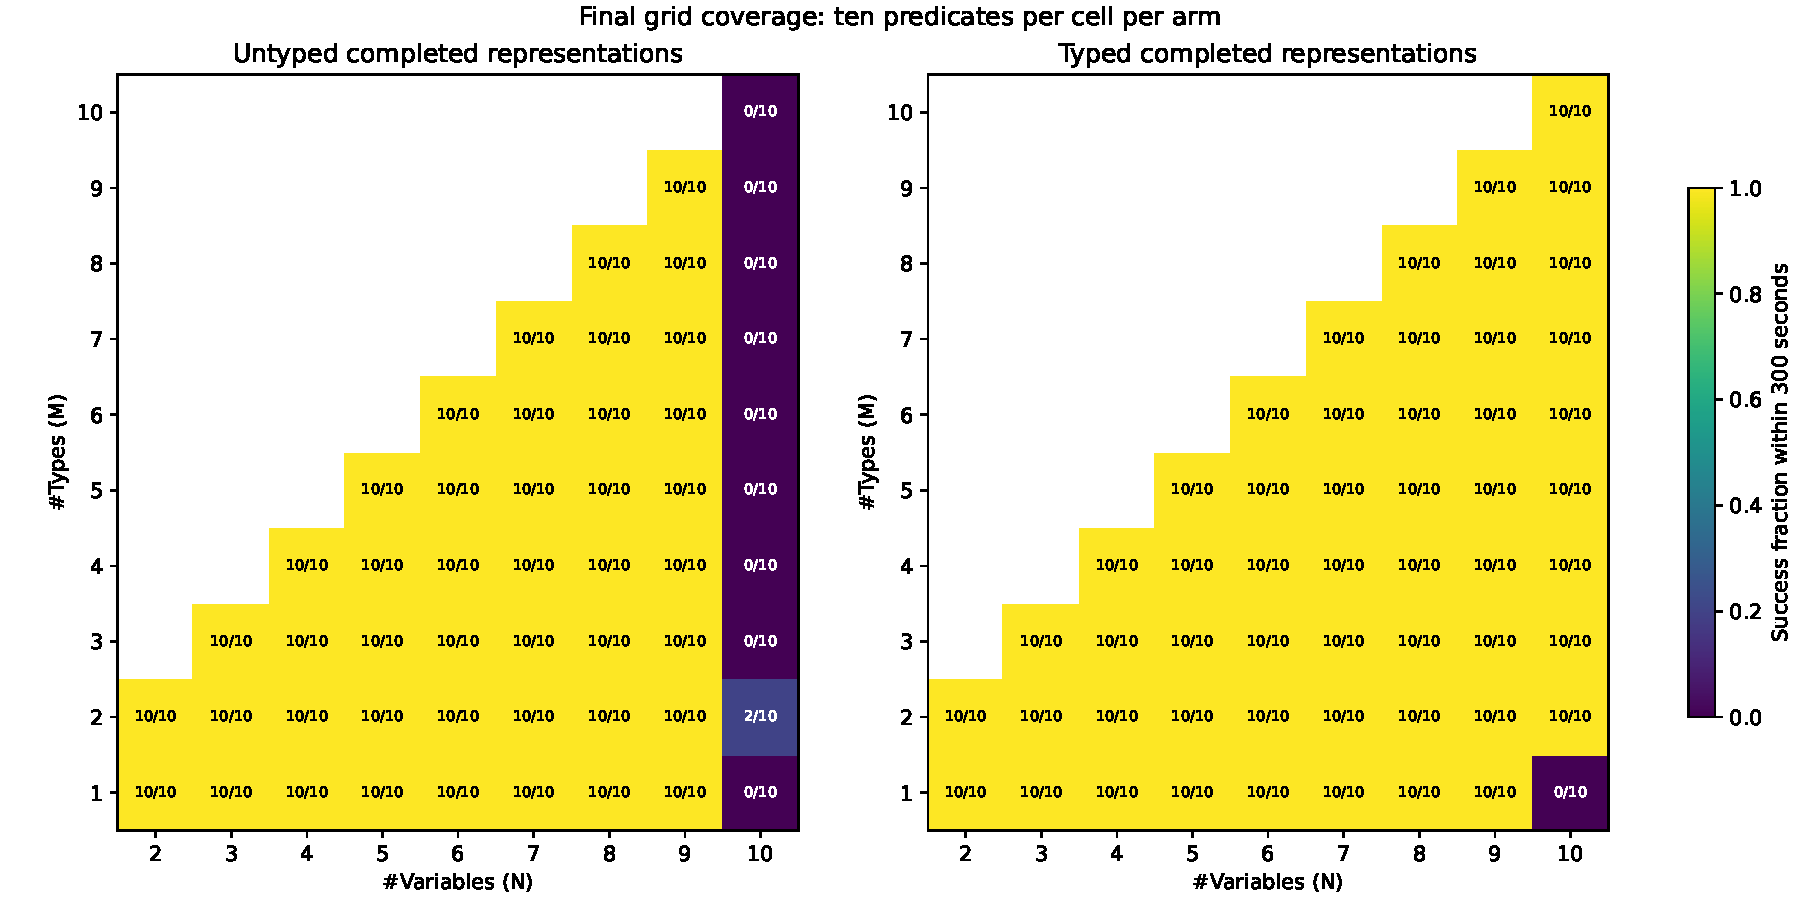
\includegraphics[width=0.94\linewidth]{figures/completion-grid.pdf}
\vspace{2pt}

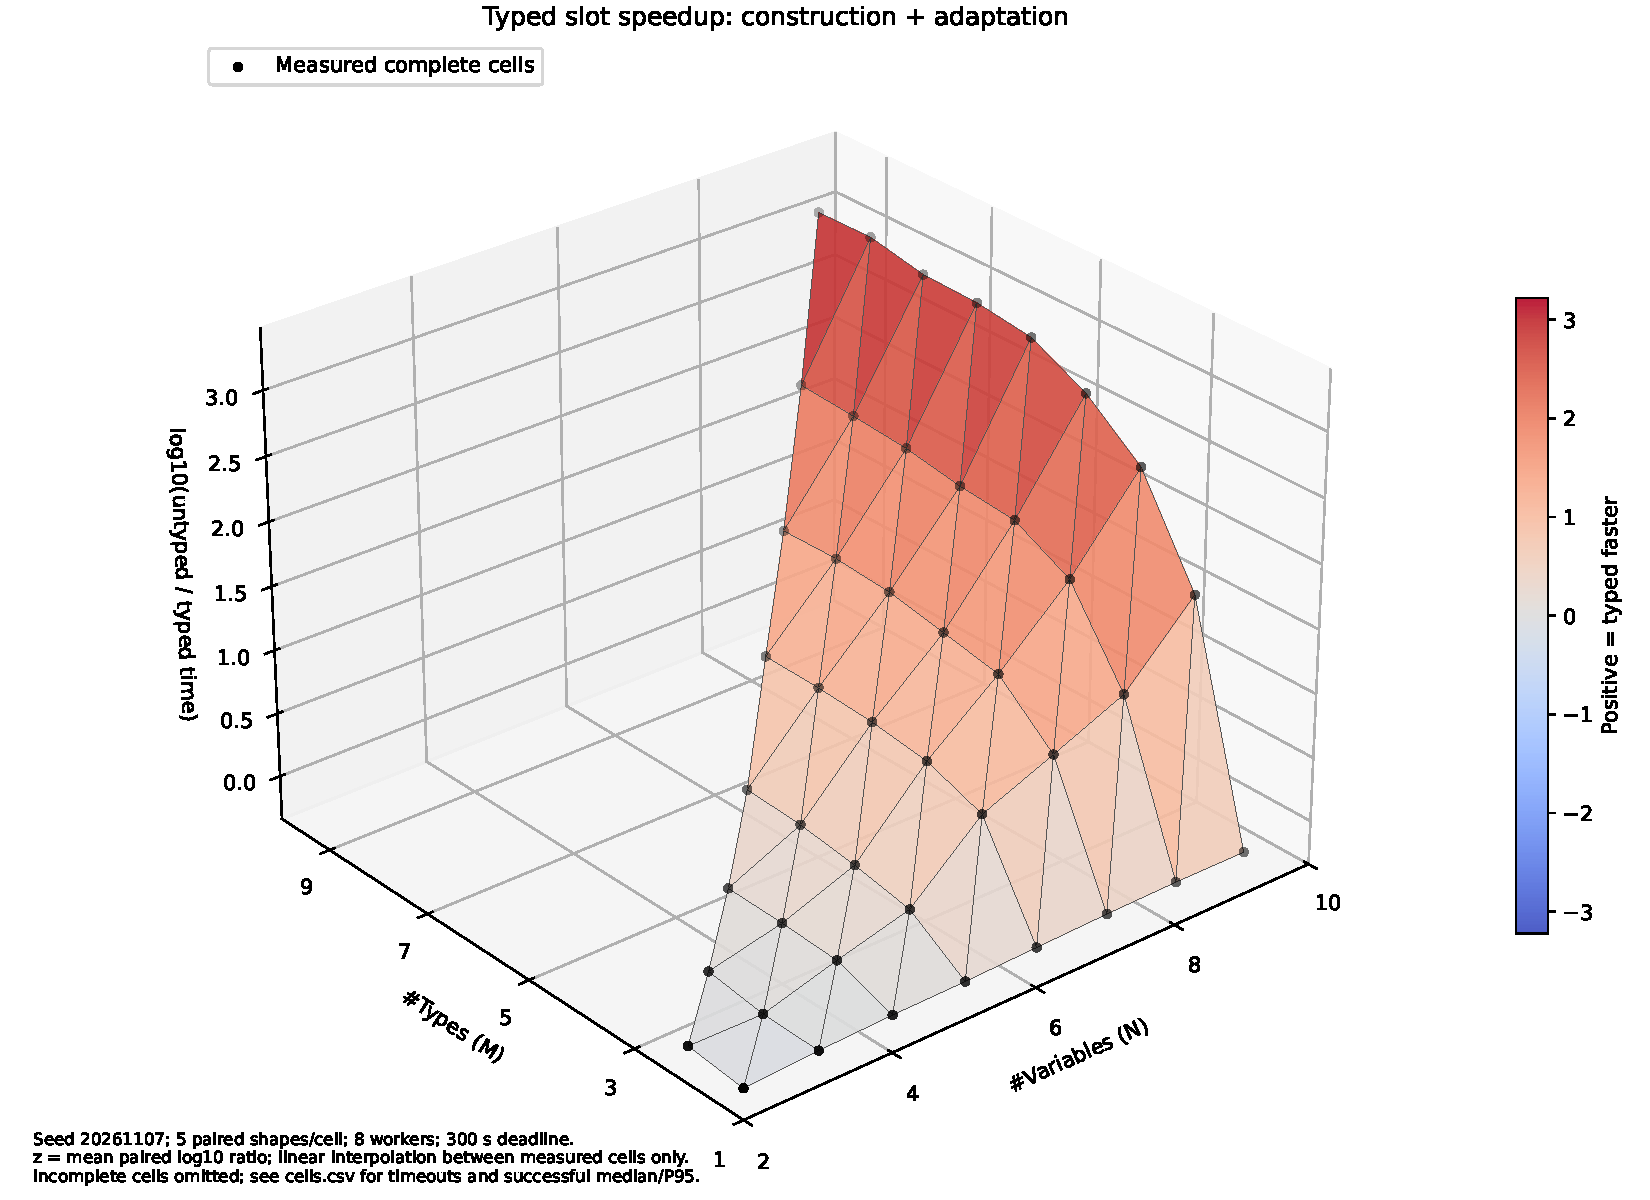
\includegraphics[width=0.72\linewidth]{figures/engine-speedup-surface.pdf}
\caption{Synthetic typed-versus-untyped scaling grid (540 predicates, 300\,s
deadline, 5 paired shapes per cell). \textbf{Top:} completion counts per
$(N,M)$ cell; all 10 typed timeouts are at $(10,1)$ and all 98 untyped timeouts
are at $N=10$. \textbf{Bottom:} mean $\log_{10}(\text{untyped}/\text{typed})$
engine elapsed time across the 44/54 complete matched cells without
interpolating across missing censored cells.}
\label{fig:synthetic-grid}
\end{figure}

On the same \textbf{442} jointly successful predicates, the ratio of untyped to
typed medians was \textbf{26.62$\times$} for engine elapsed time (0.670026\,s
vs.\ 0.025169\,s) and \textbf{5.12$\times$} for end-to-end elapsed time
(0.849457\,s vs.\ 0.166021\,s). These figures are ratios of medians over the
442 matched concurrent elapsed measurements, not medians of pairwise speedups,
CPU times, or timeout-inclusive estimates. Figure~\ref{fig:synthetic-grid}
displays the completion grid and the engine speedup surface across the 44/54
complete matched cells without interpolating missing cells (the end-to-end
surface and per-$N$ summary appear in Appendix~\ref{app:evaluation-detail}).

In the current natural slot-typing comparison, untyped and typed slots each recognized 2,228 pairs. Summed engine CPU time was 18.560\,s and 10.343\,s, respectively.

\subsection{What is the runtime and memory cost of certificate integration?}
\label{sec:eval-cost}

Fast Rewrite completed the natural arm in 27.910\,s with
2,059.3\,MiB maximum RSS. Certificate-Integrated took 386.579\,s
and 8,638.9\,MiB. These times cover each structural-ablation arm.
The paired and reference-pool runners also compare applicable Alloy commands.

\begin{table}[t]
\centering
\caption{Natural-ablation study runtime and memory across the five distinct
baselines and the two \CanDis{} implementations ($n=61{,}598$ eligible pairs).}
\label{tab:eval-runtime}
\scriptsize
\setlength{\tabcolsep}{2.1pt}
\begin{tabular}{@{}lrrrrr@{}}
\toprule
Arm & Arm Wall (s) & Eng.\ CPU (s) & Max File (s) & Peak Heap & Max RSS\\
& & & & (MiB) & (MiB)\\
\midrule
Raw & 17.531 & 3.842 & 0.158 & 696.1 & 1,347.6\\
Raw + De Bruijn & 17.788 & 4.862 & 0.139 & 728.8 & 1,381.8\\
Java egglog & 17.633 & 3.725 & 0.132 & 732.7 & 1,391.4\\
Java egglog + De Bruijn & 17.699 & 4.659 & 0.159 & 711.5 & 1,383.2\\
Slotted & 18.292 & 25.556 & 2.194 & 1,097.1 & 1,963.1\\
\CanDis{} (Fast Rewrite) & 27.910 & 151.309 & 0.384 & 1,027.1 & 2,059.3\\
\CanDis{} (Cert.-Integrated) & 386.579 & 5,512.368 & 3.962 & 6,303.3 & 8,638.9\\

\bottomrule
\end{tabular}
\end{table}

Table~\ref{tab:eval-runtime} reports one fresh process per arm.
The in-process checks and rebuilds give Certificate-Integrated a higher cost.
The study did not profile the share attributable to each operation.

\subsection{Scope and limitations}
\label{sec:eval-limits}

The Lean results address the abstract graph model. The Java results are
supported by in-process certificate checks, bounded native-operation
comparisons and the archived Alloy checks. Public operation witnesses and
end-to-end Java-to-Lean refinement remain open. The inherited labels and
recorded bounds limit the Alloy case study. The corpus contains 4,482
AST-identical paired rows and 21 cross-file raw-AST-identical reference
comparisons outside the distance measurements. Fresh-process timing
comes from a single run per ablation arm. The historical synthetic grid
preserves censored observations in cells where a trial reached its deadline.
